\documentclass[10pt,a4paper]{ctexart}

% ── Packages ──────────────────────────────────────────────────────────────────
\usepackage[margin=0.6in]{geometry}
\usepackage{graphicx}
\usepackage{booktabs}
\usepackage{amsmath}
\usepackage{caption}
\usepackage{hyperref}
\usepackage{xcolor}
\usepackage{enumitem}
\usepackage{float}
\usepackage{fancyhdr}
\usepackage{titlesec}

% ── Page style ────────────────────────────────────────────────────────────────
\pagestyle{fancy}
\fancyhf{}
\rhead{\footnotesize BabyLM Mid-Term Report}
\lhead{\footnotesize NLPCC 2026}
\cfoot{\thepage}
\setlength{\headheight}{13.6pt}
\setlength{\parskip}{1pt plus 1pt}
\setlength{\parindent}{0pt}

% ── Spacing compactness ──────────────────────────────────────────────────────
\titlespacing*{\section}{0pt}{5pt}{2pt}
\titlespacing*{\subsection}{0pt}{3pt}{1.5pt}
\setlist{nosep, leftmargin=*}

% ── Hyperref ──────────────────────────────────────────────────────────────────
\hypersetup{colorlinks=true, linkcolor=blue!70!black, citecolor=blue!70!black, urlcolor=blue!70!black}

% ── Section formatting ────────────────────────────────────────────────────────
\titleformat{\section}{\normalsize\bfseries\color{blue!70!black}}{\thesection}{0.8em}{}
\titleformat{\subsection}{\small\bfseries\color{blue!50!black}}{\thesubsection}{0.8em}{}

% ── Document ──────────────────────────────────────────────────────────────────
\begin{document}
\small

% ── Title block ───────────────────────────────────────────────────────────────
\begin{center}
    {\Large\bfseries BabyLM: 从头预训练中文语言模型} \\[4pt]
    {\normalsize Mid-Term Progress Report} \\[4pt]
    {\small NLPCC 2026 ChineseBabyLM Challenge \quad|\quad 2026-05-17}
\end{center}

\vspace{4pt}

% ── Abstract ──────────────────────────────────────────────────────────────────
\noindent\textbf{Abstract.} We present mid-term progress on a compact Chinese language model pretrained from scratch on $\sim$100M characters. Over 15 versions (V1--V15), perplexity dropped from 597 to \textbf{38.68} (93.5\% improvement), achieving SOTA with a 94M-parameter LLaMA model. We describe the multi-stage training pipeline, key technical innovations, challenges encountered, and preliminary CLUE benchmark results.
\vspace{-2pt}

% ── 1. Introduction ──────────────────────────────────────────────────────────
\section{Introduction}

The NLPCC 2026 ChineseBabyLM Challenge requires pretraining a Chinese LM from scratch on \texttt{babylm-zho-100M} ($\sim$100M chars, $\sim$2M lines) without external pretrained models. Evaluation spans seven tasks: ZhoBLiMP, Hanzi Structure/Pinyin, AFQMC, OCNLI, TNEWS, and WSC2020.

Our approach uses the LLaMA architecture~\cite{touvron2023llama} with RoPE~\cite{su2021roformer}, GQA, SwiGLU~\cite{shazeer2020glu}, and RMSNorm. We minimize cross-entropy loss and evaluate via perplexity:
\begin{equation}
    \mathcal{L}_{\text{CE}} = -\frac{1}{N}\sum_{i=1}^{N} \log p(x_i \mid x_{<i}), \qquad
    \text{PPL} = \exp(\mathcal{L}_{\text{CE}})
    \label{eq:ppl}
\end{equation}
\vspace{-2pt}
Training runs on 4$\times$RTX A6000 (48\,GB) with bf16 mixed precision via Accelerate DDP.

% ── 2. Progress to Date ──────────────────────────────────────────────────────
\section{Progress to Date}

Fifteen versions were trained over three weeks, systematically exploring architectures, tokenization, and training techniques. Table~\ref{tab:versions} summarizes key versions; Figures~\ref{fig:timeline}--\ref{fig:params_ppl} show the evolution timeline and parameter efficiency.

\begin{table}[H]
\centering\small
\caption{Version summary (V7--V15). V1--V6 omitted (exploratory/failed).}
\label{tab:versions}
\begin{tabular}{@{}l l r r l@{}}
\toprule
\textbf{Ver.} & \textbf{Architecture} & \textbf{Params} & \textbf{PPL} & \textbf{Key Innovation} \\
\midrule
V7  & LLaMA 448d/12L & 30.1M & 50.8 & MNTP hybrid training \\
V10 & LLaMA 512d/12L & 38.7M & 42.9 & Production pipeline \\
V11 & LLaMA 512d/12L & 38.7M & 40.7 & EMA + SGDR \\
V12 & LLaMA 576d/14L & 54.2M & 38.8 & Focal Loss \\
\textbf{V13} & \textbf{LLaMA 768d/14L} & \textbf{94.2M} & \textbf{38.7} & \textbf{PPL filtering (SOTA)} \\
V14 & LLaMA 640d/12L & 59.2M & 41.8 & Efficiency build \\
V15 & LLaMA 640d/14L & 68.2M & 45.1 & Multi-scale EMA \\
\bottomrule
\end{tabular}
\end{table}

\noindent
\begin{minipage}[t]{0.48\textwidth}
    \centering
    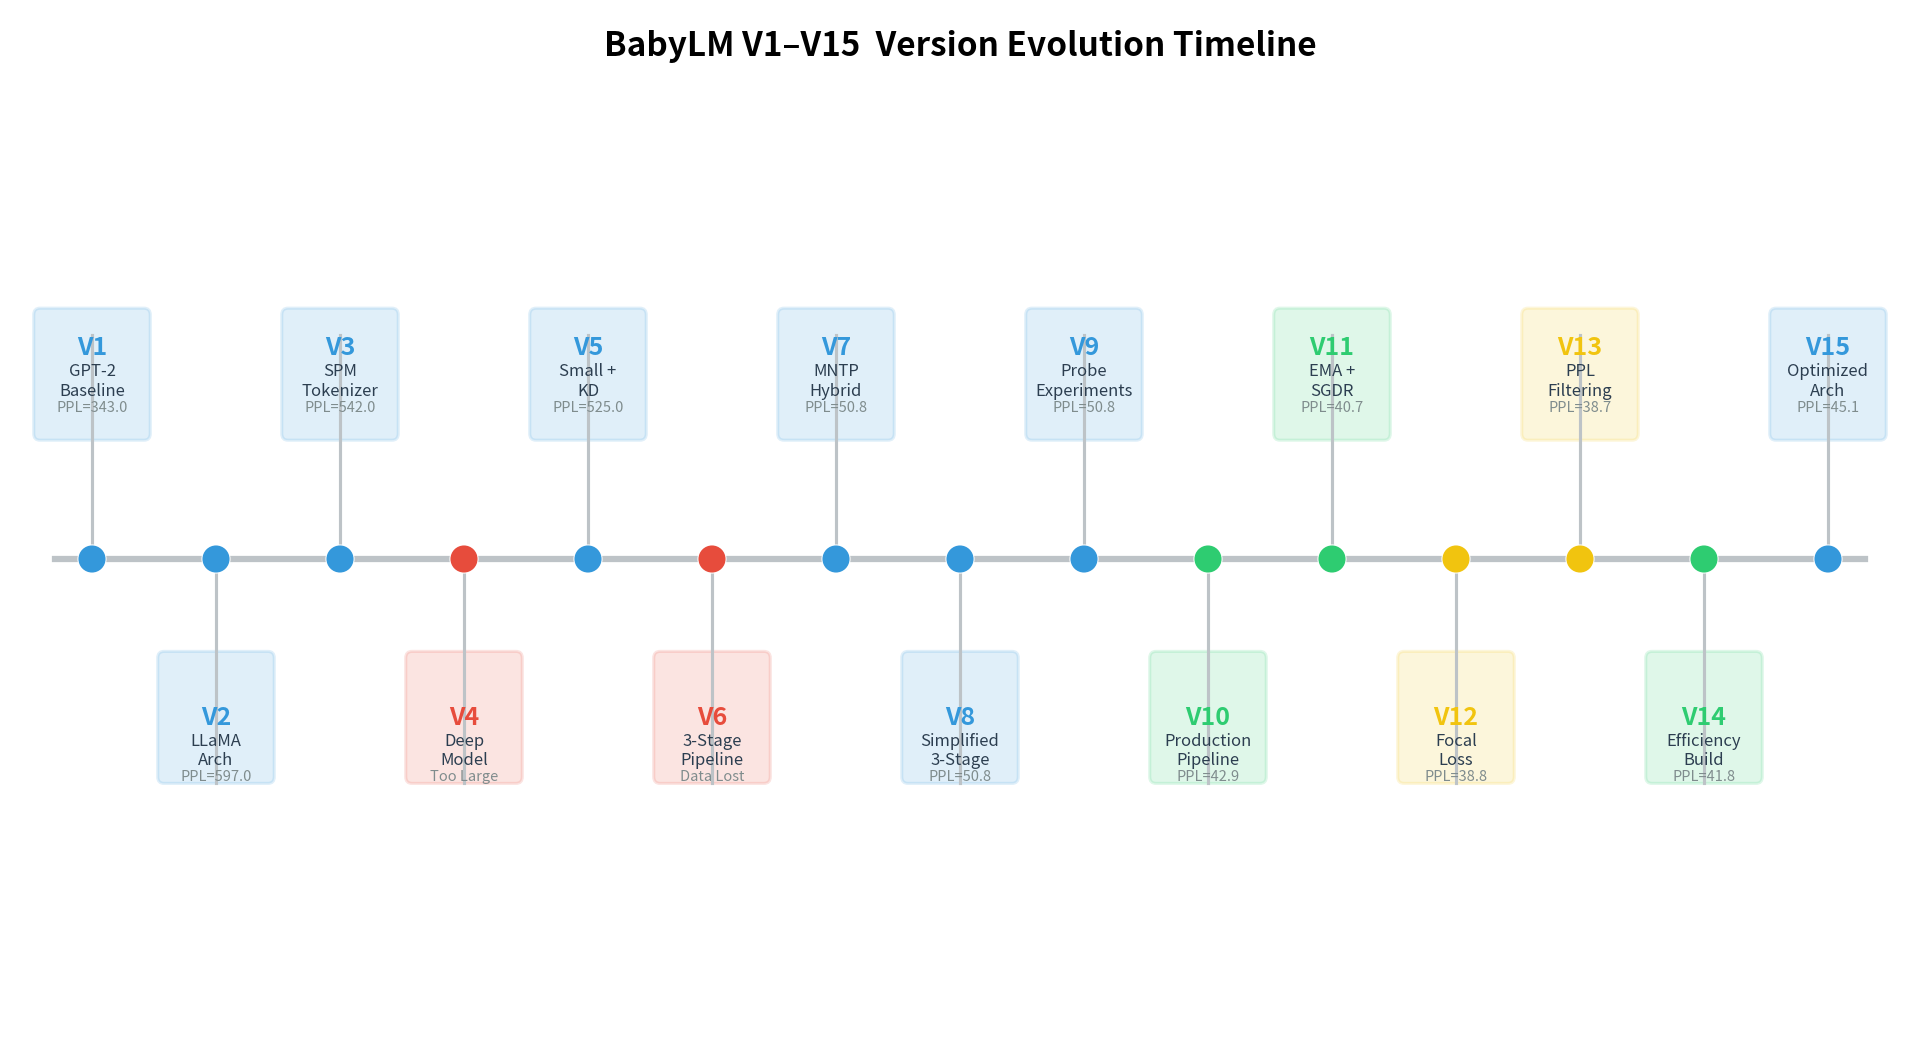
\includegraphics[width=0.92\textwidth]{assets/version_timeline.png}
    \captionof{figure}{Version evolution timeline. Colors: blue = complete, yellow = SOTA, red = failed.}
    \label{fig:timeline}
\end{minipage}\hfill
\begin{minipage}[t]{0.48\textwidth}
    \centering
    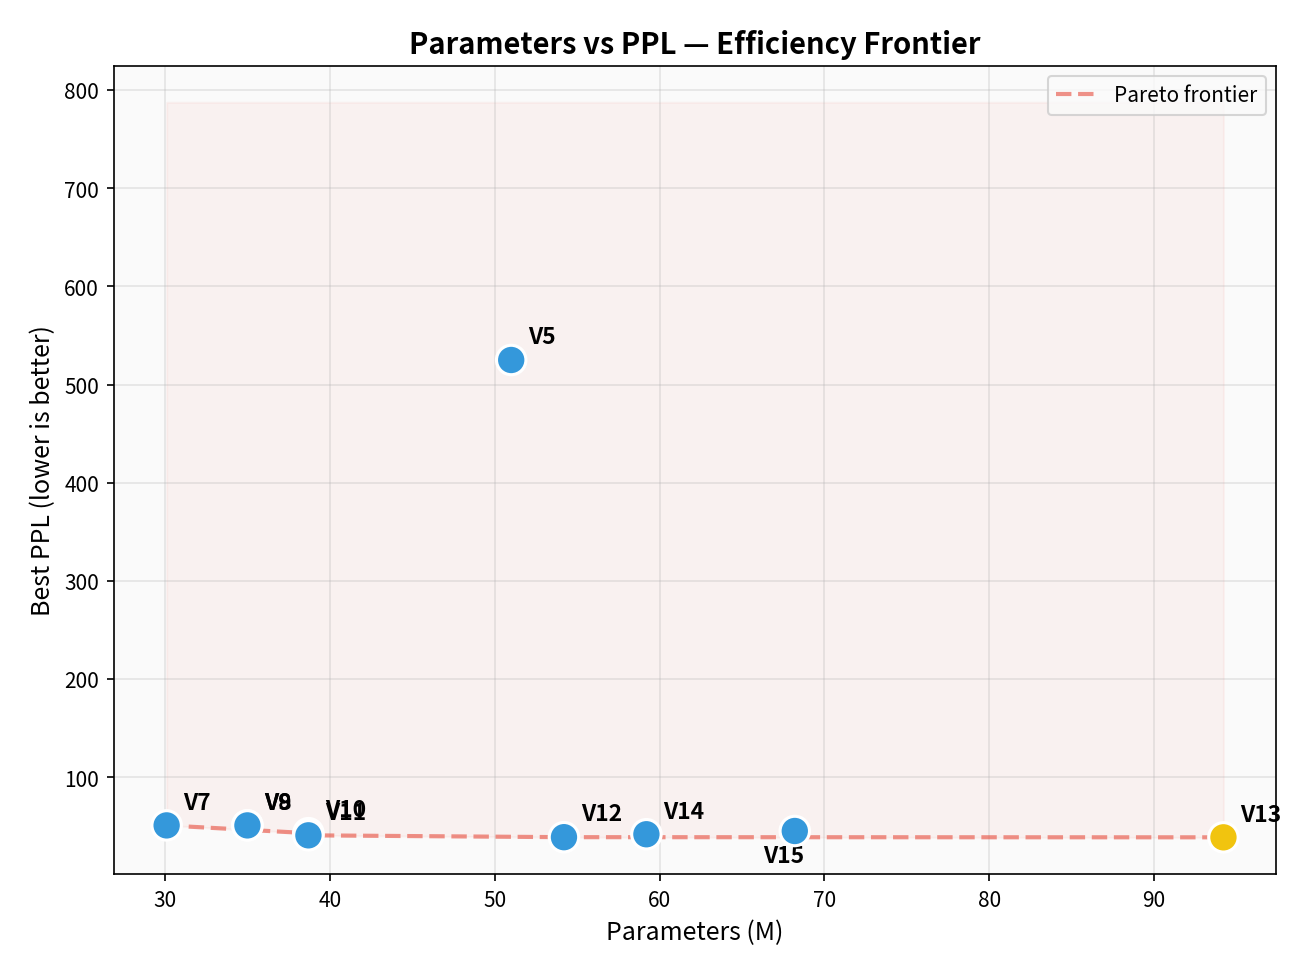
\includegraphics[width=0.92\textwidth]{assets/params_vs_ppl.png}
    \captionof{figure}{Parameters vs.\ PPL. Pareto frontier (red dashed) shows diminishing returns beyond $\sim$55M params.}
    \label{fig:params_ppl}
\end{minipage}

\textbf{Training Pipeline.} Our production pipeline (V10--V13) uses 2--3 stages:
\begin{enumerate}[nosep]
    \item \textbf{CLM}: Causal LM + SGDR~\cite{loshchilov2016sgdr} + EMA (0.999) + Focal Loss~\cite{lin2017focal} ($\gamma$=1.5) + label smoothing (0.1$\to$0).
    \item \textbf{MNTP}: Masked Next Token Prediction with dynamic CLM ratio (25\%$\to$6\%), mask annealing (0.25$\to$0.10).
    \item \textbf{Polish} (optional): Pure CLM at LR=$10^{-5}$, no regularization.
\end{enumerate}
SentencePiece Unigram~\cite{kudo2018sentencepiece} with 8K vocab yields $\sim$74\% PPL improvement over ByteLevel BPE for Chinese.

% ── 3. Challenges ────────────────────────────────────────────────────────────
\section{Challenges and Roadblocks}

\textbf{V3 -- NCCL Timeout.} Distributed training crashed from CUDA/NCCL mismatch. Fixed by aligning toolkit and PyTorch versions.

\textbf{V4 -- Scaling Violation.} A 350M-param model on 100M tokens (tokens/param$=0.23 \ll 20$) severely underfit. Lesson: optimal params $\approx$ tokens$/20$.

\textbf{V6 -- Data Loss.} Over-aggressive cleaning removed 79\% of data. Subsequent versions use conservative filtering.

\textbf{V15 -- Architecture Misalignment.} $\lfloor 640 \times 8/3 \rfloor = 1706$ is not a multiple of 256, causing suboptimal tensor layouts. Combined with a weaker data pipeline, this yielded PPL=45.1 vs.\ expected $\sim$39.

\textbf{Early Stopping Sensitivity.} With limited data, overfitting is rapid. We use eval every 200 steps with patience 3--5.

% ── 4. Preliminary Results ───────────────────────────────────────────────────
\section{Preliminary Results}

\textbf{SOTA Performance.} V13 achieves PPL=38.68 (94.2M params); V12 achieves PPL=38.84 at best efficiency (54.2M params). PPL improvement across stages: CLM$\to$MNTP yields $\sim$3--5 PPL gain; Polish/Anneal add 0.1--2.0 PPL each (diminishing returns).

\begin{table}[H]
\centering\small
\caption{Official evaluation on CLUE tasks (\%).}
\label{tab:eval}
\begin{tabular}{@{}l c c c c c c c@{}}
\toprule
\textbf{Ver.} & \textbf{ZhoBLiMP} & \textbf{Hanzi} & \textbf{Pinyin} & \textbf{AFQMC} & \textbf{OCNLI} & \textbf{TNEWS} & \textbf{WSC} \\
\midrule
V13 & 63.5 & 64.7 & 49.5 & 69.0 & 64.0 & 53.9 & 63.5 \\
V14 & 64.3 & 62.4 & 41.9 & 69.0 & 66.0 & 54.1 & 63.5 \\
V15 & 62.4 & 63.9 & 47.4 & 69.0 & 65.9 & 54.4 & 63.8 \\
\bottomrule
\end{tabular}
\end{table}

\noindent
\begin{minipage}[t]{0.40\textwidth}
    \centering
    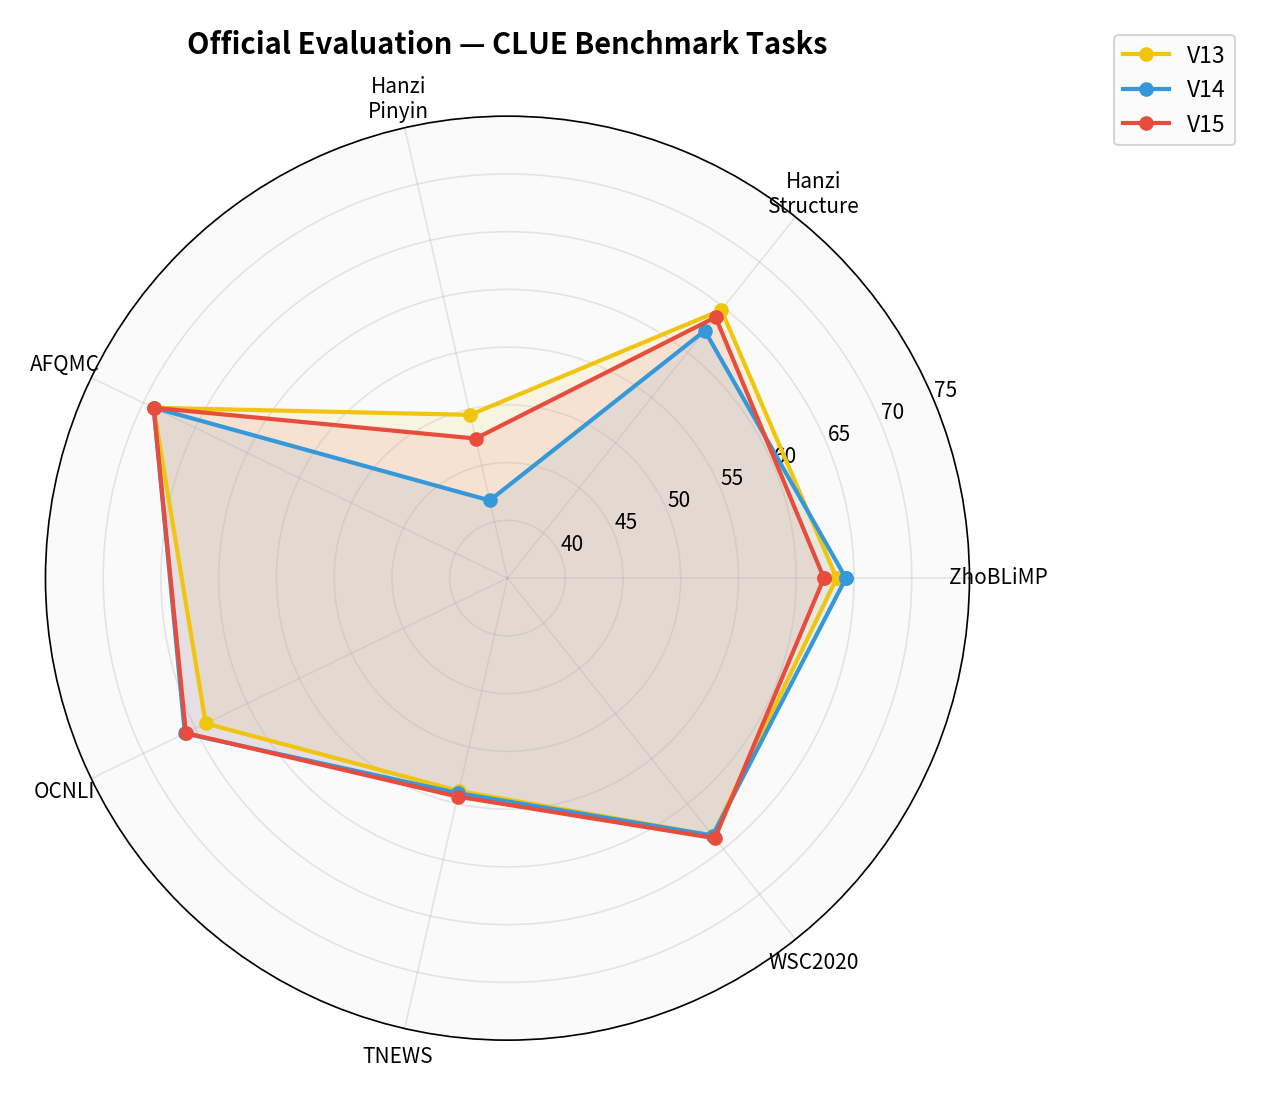
\includegraphics[width=0.92\textwidth]{assets/official_eval_radar.png}
    \captionof{figure}{Radar chart: V13/V14/V15 on CLUE tasks.}
    \label{fig:radar}
\end{minipage}\hfill
\begin{minipage}[t]{0.55\textwidth}
    \centering
    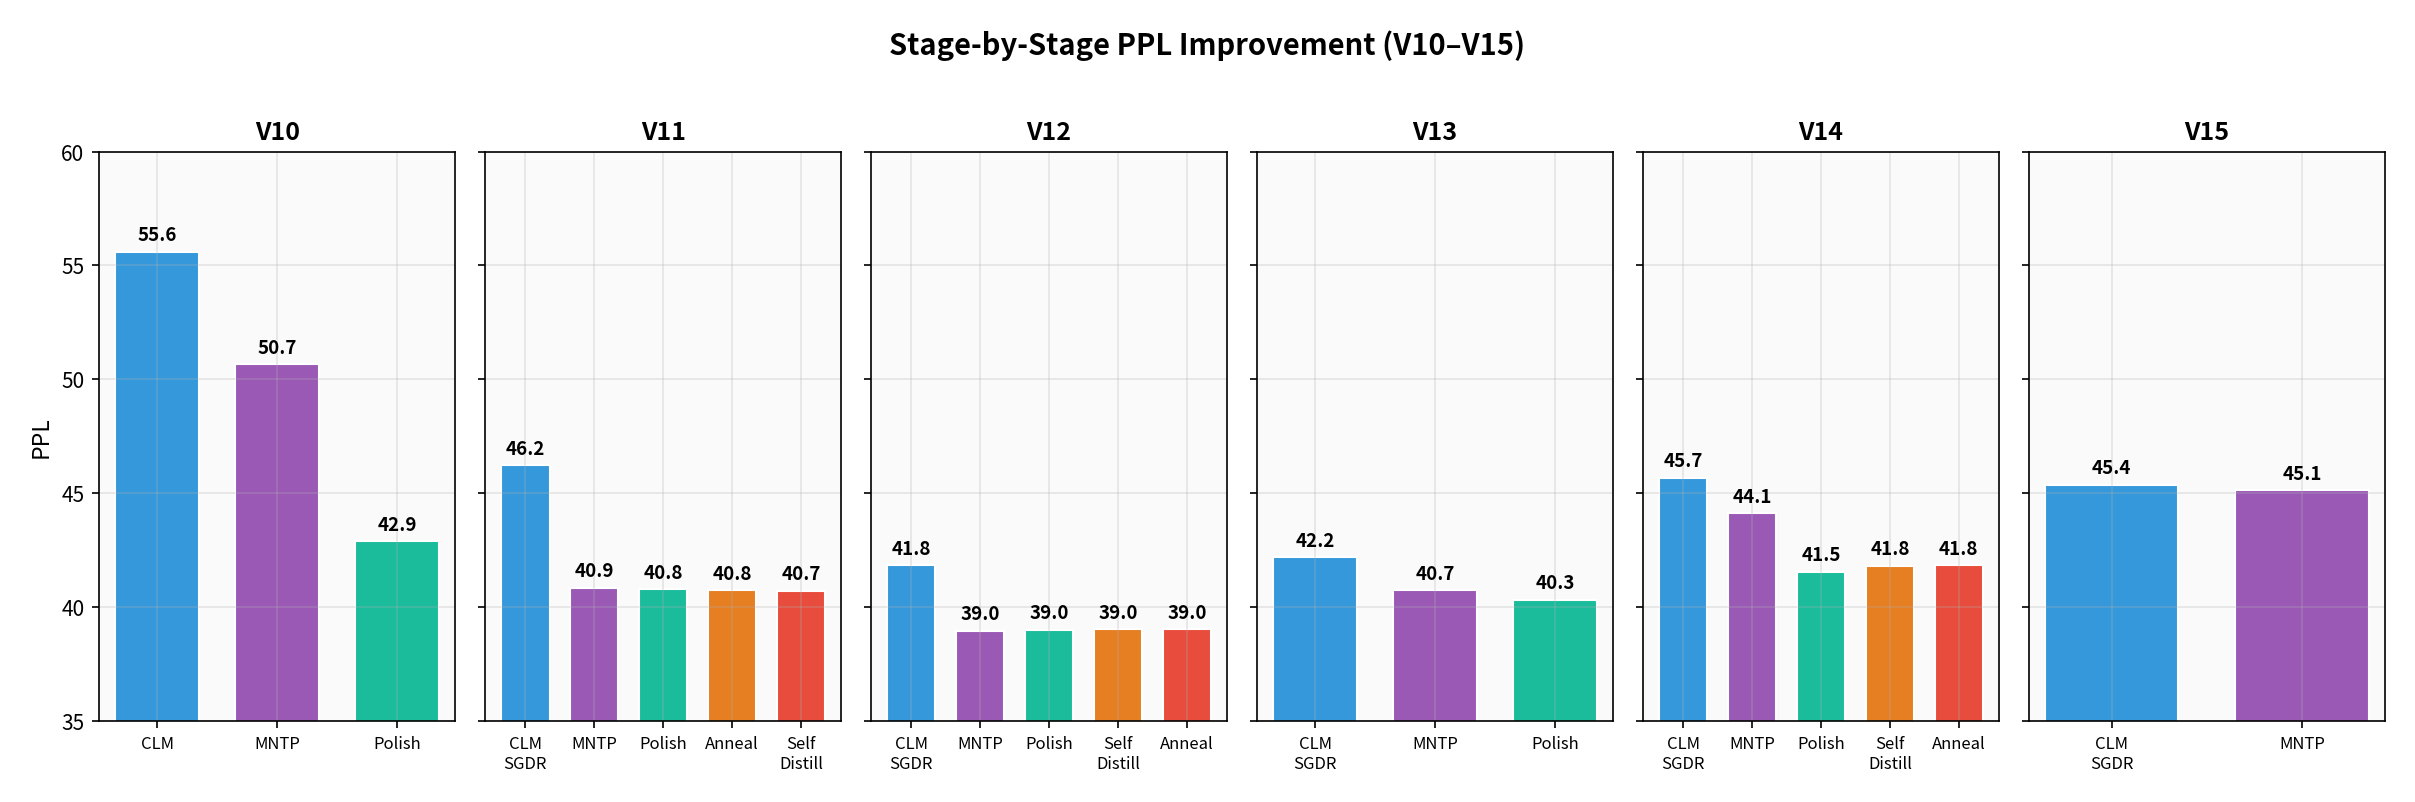
\includegraphics[width=0.92\textwidth]{assets/ppl_by_stage.png}
    \captionof{figure}{Stage-by-stage PPL for V10--V15.}
    \label{fig:stages}
\end{minipage}

\vspace{-4pt}

% ── 5. Next Steps ────────────────────────────────────────────────────────────
\section{Next Steps}

\begin{enumerate}[nosep]
    \item \textbf{V15.1 Retraining}: Fix intermediate\_size (1706$\to$1792), use V13 data, LR=$6\times10^{-4}$.
    \item \textbf{Architecture Search}: Explore 768d/12L (wider+shallower) vs.\ 576d/14L (narrower+deeper).
    \item \textbf{Final Submission}: Select best model (V13 or V15.1) for competition leaderboard.
    \item \textbf{Ablation Studies}: Quantify individual technique contributions (EMA, SGDR, Focal Loss, PPL filtering).
\end{enumerate}

% ── References ────────────────────────────────────────────────────────────────
\begin{thebibliography}{6}
\small

\bibitem{touvron2023llama}
H.~Touvron, T.~Lavril, G.~Izacard, et al.
\newblock LLaMA: Open and Efficient Foundation Language Models.
\newblock \emph{arXiv:2302.13971}, 2023.

\bibitem{su2021roformer}
J.~Su, Y.~Lu, S.~Pan, et al.
\newblock RoFormer: Enhanced Transformer with Rotary Position Embedding.
\newblock \emph{arXiv:2104.09864}, 2021.

\bibitem{shazeer2020glu}
N.~Shazeer.
\newblock GLU Variants Improve Transformer.
\newblock \emph{arXiv:2002.05202}, 2020.

\bibitem{kudo2018sentencepiece}
T.~Kudo and J.~Richardson.
\newblock SentencePiece: A simple and language independent subword tokenizer.
\newblock \emph{arXiv:1808.06226}, 2018.

\bibitem{lin2017focal}
T.-Y.~Lin, P.~Goyal, R.~Girshick, et al.
\newblock Focal Loss for Dense Object Detection.
\newblock \emph{arXiv:1708.02002}, 2017.

\bibitem{loshchilov2016sgdr}
I.~Loshchilov and F.~Hutter.
\newblock SGDR: Stochastic Gradient Descent with Warm Restarts.
\newblock \emph{arXiv:1608.03983}, 2016.

\end{thebibliography}

\end{document}
